\chapter{Risk Propagation}\label{ch:risk-propagation}

Risk propagation is a message-passing algorithm that estimates an individual's infection risk by considering their demographics, symptoms, diagnosis, and contact with others. Formally, a \define{risk score} $\vScore_t$ is a timestamped infection probability where $\vScore \in [0, 1]$ and $t \in \naturals$ is the time of its computation. Thus, an individual with a high risk score is likely to test positive for the infection and poses a significant health risk to others. There are two types of risk scores: \define{symptom scores}, or prior infection probabilities, which account for an individual's demographics, symptoms, and diagnosis \citep{Menni2020}; and \define{exposure scores}, or posterior infection probabilities, which incorporate the risk of direct and indirect contact with others.

Given their recent risk scores and contacts, an individual's exposure score is derived by marginalizing over the joint infection probability distribution. Naively computing this marginalization scales exponentially with the number of variables (i.e., individuals). To circumvent this intractability, the joint distribution is modeled as a factor graph, and an efficient message-passing procedure is employed to compute the marginal probabilities with a time complexity that scales linearly in the number of factor nodes (i.e., contacts).

Let $\vGraph = (\vVariables, \vFactors, \vEdges)$ be a \define{factor graph} where $\vVariables$ is the set of variable nodes, $\vFactors$ is the set of factor nodes, and $\vEdges$ is the set of edges incident between them \citep{Kschischang2001}. 

A \define{variable node} $\vVariable: \eventSpace \rightarrow \{0, 1\} $ is a random variable that represents the infection status of an individual, where the sample space is $\eventSpace = \{\var{healthy}, \var{infected}\}$ and
\begin{equation*}
  \vVariable(\event) =
    \begin{cases}
      0 & \text{if } \event = \var{healthy} \\
      1 & \text{if } \event = \var{infected}.
    \end{cases}
\end{equation*}
Thus, $\pr{\vVariable[i]}[t] = \vScore_t$ is a risk score of \indexed{i}{individual}.

A \define{factor node} $\vFactor: \vVariables \times \vVariables \rightarrow [0, 1]$ defines the transmission of infection risk between two contacts. Specifically, contact between \twoindexed{i}{j}{individual} is represented by the factor node $\vFactor(\vVariable[i], \vVariable[j])$ = $\vFactor[ij]$, which is adjacent to the variable nodes $\vVariable[i], \vVariable[j]$. This work and \citet{Ayday2021} assume risk transmission is a symmetric function, $\vFactor[ij] = \vFactor[ji]$. However, it may be extended to account for an individual's susceptibility and transmissibility such that $\vFactor[ij] \neq \vFactor[ji]$. \Cref{fig:factor-graph} depicts a factor graph that reflects the domain constraints.

\begin{figure}[htb]
\centering
\begin{tikzpicture}[ampersand replacement=\&]
  \matrix[row sep=1.5em, column sep=0.75em] {
    \& \factor[minimum size=1em] {f12} {above:$\vFactor[12]$} {} {}; \&\&
    \factor[minimum size=1em] {f23} {above:$\vFactor[23]$} {} {}; \& \\
    \node[latent, minimum size=2em] (v1) {$\vVariable[1]$}; \&\&
    \node[latent, minimum size=2em] (v2) {$\vVariable[2]$}; \&\&
    \node[latent, minimum size=2em] (v3) {$\vVariable[3]$}; \\
  };
  \edge[-] {v1} {f12};
  \edge[-] {v2} {f12};
  \edge[-] {v2} {f23};
  \edge[-] {v3} {f23};
\end{tikzpicture}
\caption[Factor graph]{A factor graph of 3 variable nodes and 2 factor nodes.}
\label{fig:factor-graph}
\end{figure}

\section{Synchronous Risk Propagation}\label{sec:synchronous}

\newcommand{\pDiff}{\epsilon}
\newcommand{\topK}[1]{\text{top } K \text{ of } #1}
\newcommand{\vRiskScores}[2]{\vSet{R}_{#1}^{(#2)}}
\newcommand{\vExposureScore}[2]{r_{#1}^{(#2)}}
\newcommand{\vExposureScores}[1]{\mathbf{r}^{(#1)}}
\newcommand{\dist}{d}

\citet{Ayday2021} first proposed risk propagation as a synchronous, iterative message-passing algorithm that uses the factor graph to compute exposure scores. The first input to \cRiskPropagation{} is the set family $\vScores$, where
\begin{equation} \label{eq:score-set}
  \vScores_i =\setBuilder{\vScore_t}{\vRefTime - t < \pScoreExpiry} \in \vScores
\end{equation}
is the set of recent risk scores of \indexed{i}{individual}. The second input to \cRiskPropagation{} is the contact set
\begin{equation} \label{eq:contact-set}
  \vContacts = \setBuilder{(i, j, t)}{i \neq j, \vRefTime - t < \pContactExpiry}
\end{equation}
such that $(i, j, t)$ is the \emph{most recent} contact between \twoindexed{i}{j}{individual} that occurred from time $t$ until at least time $t + \pMinContactDuration$, where $\pMinContactDuration \in \naturals$ is the \define{minimum contact duration}\footnote{While \citet{Ayday2021} require contact over a $\pMinContactDuration$-contiguous period of time, the Centers for Disease Control and Prevention \citeyearpar{CDC2021} account for contact over a 24-hour period.}. Naturally, risk scores and contacts have finite relevance, so \eqref{eq:score-set} and \eqref{eq:contact-set} are constrained by the \define{risk score expiry} $\pScoreExpiry \in \naturals$ and the \define{contact expiry} $\pContactExpiry \in \naturals$, respectively. The \define{reference time} $\vRefTime \in \naturals$ defines the relevance of the inputs and is assumed to be the time at which \cRiskPropagation{} is invoked. For notational simplicity in \cRiskPropagation{}, let $\vSomeSet$ be a set. Then $\max \vSomeSet = 0$ if $\vSomeSet = \emptyset$.

\subsection{Variable Messages}

The current exposure score of \indexed{i}{individual} is defined as $\max \vScores_i$. Hence, a \define{variable message} $\vVariableMessage{i}{j}{n}$ from the variable node $\vVariable[i]$ to the factor node $\vFactor[ij]$ during \indexed{n}{iteration} is the set of maximal risk scores $\vRiskScores{i}{n - 1}$ from the previous $n - 1$ iterations that were not derived by $\vFactor[ij]$. In this way, risk propagation is reminiscent of the max-sum algorithm; however, risk propagation aims to maximize \emph{individual} marginal probabilities rather than the joint distribution \cite[pp. 411--415]{Bishop2006}.

\subsection{Factor Messages}

A \define{factor message} $\vFactorMessage{i}{j}{n}$ from the factor node $\vFactor[ij]$ to the variable node $\vVariable[j]$ during \indexed{n}{iteration} is an exposure score of \indexed{j}{individual} that is based on interacting with those at most $n - 1$ degrees separated from \indexed{i}{individual}. This population is defined by the subgraph induced in $\vGraph$ by
\begin{equation*}
  \setBuilder{v \in \vVariables \cap \vFactors \setminus \{\vVariable[j], \vFactor[ij]\}}{\dist(\vVariable[i], v) \leq 2(n - 1)},
\end{equation*}
where $\dist(u, v)$ is the distance between the nodes $u, v$. The computation of a factor message assumes the following.
\begin{enumerate}
  \item Contacts have a nondecreasing effect on an individual's exposure score.
  \item A risk score $\vScore_t$ is \define{relevant} to the contact $(i, j, t_{ij})$ if $t < t_{ij} +\pTimeBuffer$, where $\pTimeBuffer \in \naturals$ is a \define{time buffer} that accounts for the incubation period, along with the delayed reporting of symptom scores and contacts. The expression $t_{ij} +\pTimeBuffer$ is called the \define{buffered contact time}.
  \item Risk transmission between contacts is incomplete. Thus, a risk score decays exponentially along its transmission path in $\vGraph$ at a rate of $\log \pTransmissionRate$, where $\pTransmissionRate \in (0, 1)$ is the \define{transmission rate}.
\end{enumerate}
To summarize, a factor message $\vFactorMessage{i}{j}{n}$ is the maximum relevant risk score in the variable message $\vVariableMessage{i}{j}{n}$ (or 0) that is scaled by the transmission rate $\pTransmissionRate$.

\citet{Ayday2021} assume that the contact set $\vContacts$ may contain (1) multiple contacts between the same two individuals and (2) \define{invalid} contacts, or those lasting less than $\pMinContactDuration$ time. However, these assumptions introduce unnecessary complexity. Regarding assumption 1, suppose \twoindexed{i}{j}{individual} come into contact $m$ times such that $t_k < t_\ell$ for $1 \leq k < \ell \leq m$. Let $\vFactorMessages_k$ be the set of relevant risk scores, according to the contact time $t_k$, where
\begin{equation*}
  \vFactorMessages_k = \setBuilder{\pTransmissionRate \vScore_t}{\vScore_t \in \vVariableMessage{i}{j}{n}, t < t_k + \pTimeBuffer}.
\end{equation*}
Then $\vFactorMessages_k \subseteq \vFactorMessages_\ell$ if and only if $\max \vFactorMessages_k \leq \max \vFactorMessages_\ell$. Therefore, only the most recent contact time $t_m$ is required to compute the factor message $\vFactorMessage{i}{j}{n}$. With respect to assumption 2, there are two possibilities.
\begin{enumerate}
  \item If an individual has at least one valid contact, then their exposure score is computed over the subgraph induced in $\vGraph$ by their contacts that define the neighborhood $\vNeighbors_i$ of the variable node $\vVariable_i$.
  \item If an individual has no valid contacts, then their exposure score is $\max \vScores_i$ or $0$, if all of their previously computed risk scores have expired.
\end{enumerate}
In either case, a set $\vContacts$ containing only valid contacts implies fewer factor nodes and edges in the factor graph $\vGraph$. Consequently, the complexity of \cRiskPropagation{} is reduced by a constant factor since fewer messages must be computed.

\subsection{Termination}

To detect convergence, the normed difference between the current and previous exposure scores is compared to the threshold $\pDiff \in \reals$. Note that $\vExposureScores{n}$ is the vector of exposure scores in the \indexed{n}{iteration} such that $\vExposureScore{i}{n}$ is \indexed{i}{component} of $\vExposureScores{n}$. The $\ell^1$ and $\ell^\infty$ norms are sensible choices for detecting convergence. \citet{Ayday2021} use the $\ell^1$ norm, which ensures that an individual's exposure score changed by at most $\pDiff$ after the penultimate iteration.

\begin{function}[H]{\nRiskPropagation}[\vScores, \vContacts]
  \State $(\vVariables, \vFactors, \vEdges) \assign \cCreateFactorGraph[\vContacts]$
  \State $n \assign 1$
  \ForEach{$\vVariable[i] \in \vVariables$}
    \State $\vRiskScores{i}{n - 1} \assign \topK{\vScores_i}$
    \State $\vExposureScore{i}{n - 1} \assign \max \vRiskScores{i}{n - 1}$
    \State $\vExposureScore{i}{n} \assign \infty$
  \EndFor
  \While{$\| \vExposureScores{n} - \vExposureScores{n - 1} \| > \pDiff$}
    \ForEach{$\{\vVariable[i], \vFactor[ij]\} \in \vEdges$}
      \State $\vVariableMessage{i}{j}{n} \assign \vRiskScores{i}{n - 1} \setminus \setBuilder{\vFactorMessage{j}{i}{k}}{k \in [1 \twodots n - 1]}$
    \EndFor
    \ForEach{$\{\vVariable[i], \vFactor[ij]\} \in \vEdges$}
      \State $\vFactorMessage{i}{j}{n} \assign \max \setBuilder{\pTransmissionRate \vScore_t}{\vScore_t \in \vVariableMessage{i}{j}{n}, t < t_{ij} + \pTimeBuffer}$
    \EndFor
    \ForEach{$\vVariable[i] \in \vVariables$}
      \State $\vRiskScores{i}{n} \assign \topK{\setBuilder{\vFactorMessage{j}{i}{n}}{\vFactor[ij] \in \vNeighbors_i}}$
    \EndFor
    \ForEach{$\vVariable[i] \in \vVariables$}
      \State $\vExposureScore{i}{n - 1} \assign \vExposureScore{i}{n}$
      \State $\vExposureScore{i}{n} \assign \max \vRiskScores{i}{n}$
    \EndFor
    \State $n \assign n + 1$
  \EndWhile
  \State \Return $\vExposureScores{n}$
\end{function}

\section{Asynchronous Risk Propagation}\label{sec:asynchronous}

While straightforward to specify, \cRiskPropagation{}, is not a viable implementation for real-world application, because it is an \define{offline algorithm} that requires all individuals' recent contacts and risk scores to run. As \citet{Ayday2021} note, the centralization of health and contact data is not privacy preserving. An offline design is also computational inefficient and risks human safety. Specifically, most exposure scores may not change across invocations of \cRiskPropagation{}, which implies communication overhead and computational redundancy. As a mitigation, \citet{Ayday2020} suggest running \cRiskPropagation{} only once or twice daily. However, this causes substantial delay in reporting to individuals their exposure scores; and in the face of a pandemic, timely information is essential for individual and collective health.

To address the privacy limitations of \cRiskPropagation{}, \citet{Ayday2021} propose decentralizing the factor graph such that the processing entity (e.g., mobile device or ``personal cloud'') associated with \indexed{i}{individual} maintains the state of \indexed{i}{variable node} and its neighboring factor nodes. But for real-world application, the proposal leaves key questions unanswered:
\begin{enumerate}
  \item Is message passing synchronous or asynchronous?
  \item How does message passing terminate?
  \item Are any optimizations utilized to reduce communication cost?
  \item How do processing entities exchange messages over the network?
  \item How private is decentralized risk propagation?
\end{enumerate}

%Key observations:
%
%- Asynchronous message passing amongst stateful entities is the essence of the actor model, so we can use it to describe risk propagation as an online algorithm
%- By applying one-mode projection, the factor graph is equivalent to a contact network. Thus, we can extend the concepts of reachability in temporal network to account for message-passing semantics and measure the communication complexity of risk propagation.

The only purpose of a factor node is to compute and relay messages between variable vertices. Thus, one-mode projection onto the variable vertices can be applied such that variable vertices $\vVariable[i],\vVariable[j] \in \vVariables$ are adjacent if the factor node $\vFactor[ij] \in \vFactors$ exists \citep{Zhou2007}. \Cref{fig:projected} shows the modified topology.

\begin{figure}[htb]
\centering
\begin{tikzpicture}[ampersand replacement=\&]
  \matrix[row sep=7em, column sep=2em] {
    \node[latent, minimum size=2em] (v1) {$\vVariable[1]$}; \&\&\&
    \node[latent, minimum size=2em] (v2) {$\vVariable[2]$}; \&\&\&
    \node[latent, minimum size=2em] (v3) {$\vVariable[3]$}; \\
  };
  \factor[minimum size=1em, above= of v1] {f12_1} {above:$\vFactor[12]$} {} {};
  \factor[minimum size=1em, above= of v2, xshift=-3em] {f12_2} {above:$\vFactor[12]$} {} {};
  \factor[minimum size=1em, above= of v2, xshift=3em] {f23_2} {above:$\vFactor[23]$} {} {};
  \factor[minimum size=1em, above= of v3] {f23_3} {above:$\vFactor[23]$} {} {};
  
  \plate{p1} {(v1)(f12_1)(f12_1-caption)} {};
  \plate{p2} {(v2)(f12_2)(f23_2)(f12_2-caption)(f23_2-caption)} {};
  \plate{p3} {(v3)(f23_3)(f23_3-caption)} {};
  
  \edge[-] {v1} {f12_1};
  \edge[-] {v2} {f12_2};
  \edge[-] {v2} {f23_2};
  \edge[-] {v3} {f23_3};
  \edge[-] {p1} {p2};
  \edge[-] {p2} {p3};
\end{tikzpicture}
\caption[One-mode projection of a factor graph]{One-mode projection onto the variable nodes in \Cref{fig:factor-graph}.}
\label{fig:projected}
\end{figure}

To send a message to variable node $\vVariable[i]$, variable node $\vVariable[j]$ applies the computation associated with the factor node $\vFactor[ij]$. This modification differs from the distributed extension of risk propagation \citep{Ayday2021} in that we do not create duplicate factor vertices and messages in each user's PDS. By storing the contact time between users on the edge incident to their variable vertices, this modified topology is identical to the \emph{contact-sequence} representation of a \emph{contact network}, a kind of \emph{time-varying} or \emph{temporal network} in which a node represents a person and an edge indicates that two persons came in contact:
\begin{equation}
  \setBuilder{(u, v, t)}{u, v \in \vVertices; u \neq v; t \in \naturals}, \label{eq:contact-seq}
\end{equation}
where a triple $(u, v, t)$ is called a \emph{contact} \citep{Holme2012}. Specific to risk propagation, $t$ is the time at which users $u$ and $v$ \emph{most recently} came in contact (see \Cref{sec:asynchronous}).

The usage of a temporal network in this work differs from its typical usage in epidemiology which focuses on modeling and analyzing the spreading dynamics of disease \citep{Riolo2001, Danon2011, Lokhov2014, Craft2015, Pastor-Satorras2015, Koher2019, Zino2021}. In contrast, this work uses a temporal network to infer a user's MPPI. As a result, \Cref{sec:reachability} extends temporal reachability to account for both the message-passing semantics and temporal dynamics of the network. As noted by \citet{Holme2012}, the transmission graph provided by \citet{Riolo2001} ``cannot handle edges where one node manages to not catch the disease.'' Notably, the usage of a temporal network in this work allows for such cases by modeling the possibility of infection as a continuous outcome.
% TODO
Factor graphs are useful for decomposing complex probability distributions and allowing for efficient inference algorithms.

However, as with risk propagation, and generally any application of a factor graph in which the variable vertices represent entities of interest (i.e., of which the marginal probability of a variable is desired), applying one-mode projection is a .

\subsection{ShareTrace Actor System}

As a distributed algorithm, risk propagation is specified from the perspective of an \emph{actor}. Some variation exists on exactly how actor behavior is defined \citep{Agha1985, Koster2016}. Perhaps the simplest definition is that the \emph{behavior of an actor} is both its \emph{interface} (i.e., the types of messages it can receive) and \emph{state} (i.e., the internal data it uses to process messages) \citep{Koster2016}. An \emph{actor system}\footnote{This is technically referred to as an \emph{actor system configuration}.} is defined as the set of actors it contains and the set of unprocessed messages\footnote{Formally, a \emph{message} is called a \emph{task} and is defined by a \emph{tag}, a unique identifier; a \emph{target}, the mail address to which the message is delivered; and a \emph{communication}, the message content \citep{Agha1985}.} in the actor mailboxes. An expanded definition of an actor system also includes a \emph{local states function} that maps mail addresses to behaviors, the set of \emph{receptionist actors} that can receive communication that is external to the actor system, and the set of \emph{external actors} that exist outside of the actor system \citep{Agha1985}. Practically, a local states function is unnecessary to specify, so the narrower definition of an actor system is used. The remainder of this section describes the components of the ShareTrace actor system.

\subsection{Actor Behavior}\label{sec:actor-behavior}

Each individual corresponds to an actor that participates in the message-passing protocol of risk propagation. Herein, the user of an actor will only be referred to as an \emph{actor}. The following variant of the concurrent, object-oriented actor model is assumed to define actor behavior \citep{Agha1985}.

\begin{itemize}
  \item An actor follows the \define{active object pattern} \citep{Lavender1996, Koster2016} and the \define{Isolated Turn Principle} \citep{Koster2016}. Specifically, the state change of an actor is carried out by instance- variable assignment, instead of the canonical \cBecome{} primitive that provides a functional construct for pipelining actor behavior replacement \citep{Agha1985}. The interface of an actor is fixed in risk propagation, so the more general semantics of \cBecome{} is unnecessary.
  \item The term ``name'' \citep{Hewitt1977, Agha1985} is preferred over ``mail address'' \citep{Agha1985} to refer to the sender of a message. Generally, the mail address that is included in a message need not correspond to the actor that sent it. Risk propagation, however, requires this actor is identified in a risk score message. Therefore, to emphasize this requirement, ``name'' is used to refer to both the identity of an actor and its mail address.
  \item An actor is allowed to include a loop with finite iteration in its behavior definition; this is traditionally prohibited in the actor model \citep{Agha1985}.
  \item The behavior definition is implied by all procedures that take as input an actor.
\end{itemize}

The \cCreateActor{} operation initializes an actor \citep{Agha1985}. An actor $\vActor$ has the following attributes.
\begin{itemize}
  \item $\aActorExposure$: the current exposure score of the individual that this actor represents. This attribute is either a symptom score, a risk score sent by another actor, or the null risk score (see \cNullRiskScore).
  \item $\aActorContacts$: a \define{dictionary} (\Cref{ch:data-structures}) that maps an actor name to a contact. In the context of an actor, a \define{contact} is a \define{proxy} \citep{Gamma1995} of the actor that represents an individual with which the individual represented by this actor was physically proximal. That is, if \indexed{i}{individual} was physically proximal to \indexed{j}{individual}, then $\aContacts{\vActor_i}$ contains a name of \indexed{j}{actor} and the most recent time of contact. This attribute extends the concept of \emph{actor acquaintances} \citep{Hewitt1977a, Hewitt1977b, Agha1985} to be time-varying.
  \item $\aActorScores$: a dictionary that maps a time interval to the maximum risk score (i.e., exposure score) received by this actor during that interval\footnote{This type of data structure is known as an \define{interval tree} and can be implemented by augmenting a red-black tree \citep[pp. 489--494]{Cormen2022}}. The null risk score is returned for queries in which the dictionary does not contain a key interval that intersects with the given query interval. \Cref{fig:exposure} depicts a hypothetical step function that $\aActorScores$ represents.
\end{itemize}

\begin{figure}[htb]
\centering
\begin{tikzpicture}
\begin{axis}[
  xlabel={Time},
  ylabel={Exposure score},
  xtick=\empty,
]
  \addplot [const plot mark right] coordinates {
    (0, 0)
    (2, 0)
    (3, 0.3)
    (6, 0.7)
    (9, 0.6)
    (11, 0.9)
    (15, 0.8)
    (17, 0.4)
  };
\end{axis}
\end{tikzpicture}
\caption[An actor's exposure score over time]{An actor's exposure score over time.}
\label{fig:exposure}
\end{figure}

\begin{function}{\nNullRiskScore}
  \State $\aScoreValue \assign 0$
  \State $\aScoreTime \assign 0$
  \State $\aScoreSender \assign \nil$
  \State \Return $\vScore$
\end{function}

\begin{function}{\nCreateActor}
  \State $\aActorContacts \assign \emptyset$
  \State $\aActorScores \assign \emptyset$
  \State $\aActorExposure \assign \cNullRiskScore$
  \State \Return $\vActor$
\end{function}

Note that \cCreateActor{} does not specify a name for the actor. This allows the actor to have multiple names and for them to be specified ``out-of-band.''

The interface of an actor is primarily defined by two types of messages: contacts and risk scores. As with \Cref{sec:synchronous}, contacts and risk scores have finite relevance. Let the \define{time-to-live} (TTL) of a message be the remaining time of its relevance. The reference time $\vRefTime$ is assumed to be the current time.

\begin{function}{\nRiskScoreTtl}[\vScore]
  \State \Return $\pScoreExpiry - (\vRefTime - \aScoreTime)$
\end{function}

\begin{function}{\nContactTtl}[\vContact]
  \State \Return $\pContactExpiry - (\vRefTime - \aContactTime)$
\end{function}

The \cHandleRiskScore{} operation defines the actions an actor performs upon receiving a risk score. The key associated with the risk score is the time interval during which it is relevant. For the dictionary $\aActorScores$, \cMerge{} preserves the mapping invariant defined above such that risk scores are ordered first by value and then by time. The \cUpdateExposureScore{} operation describes how $\aActorExposure$ is updated. Additional context is needed before specifying \cApplyRiskScore{} in detail. For now, it is sufficient to know that the operation uses the risk score to update the state of a contact.

\begin{function}{\nHandleRiskScore}[\vActor, \vScore]
  \If{$\cRiskScoreTtl[\vScore] > 0$}
    \State $\aScoreKey \assign [\aScoreTime, \aScoreTime + \pScoreExpiry)$
    \State $\cMerge[\aActorScores, \vScore]$
    \State $\cUpdateExposureScore[\vActor, \vScore]$
    \ForEach{$\vContact \in \aActorContacts$}
      \State $\cApplyRiskScore[\vActor, \vContact, \vScore]$
    \EndFor
  \EndIf
\end{function}

\begin{function}{\nUpdateExposureScore}[\vActor, \vScore]
  \If{$\aActorExposureValue < \aScoreValue$}
    \State $\aActorExposure \assign \vScore$
  \ElsIf{$\cRiskScoreTtl[\aActorExposure] \leq 0$}
    \State $\aActorExposure \assign \cMaximum[\aActorScores]$
  \EndIf
\end{function}

% Message optimizations - sender-side aggregation with flush timeouts
% Message passing termination - send coefficient and send threshold

% Contact (actor context) - a remote proxy of an actor that represents an individual with which the individual represented by the present actor came into physical proximity; a message filter and aggregator; employs sender-side aggregation (a message-passing optimization) to reduce communication complexity.

%In previous work \citep{Ayday2021}, risk propagation assumes synchronous message passing, so the notion of an iteration or inter-iteration difference threshold can be used as stopping conditions. However, as a streaming algorithm that relies on asynchronous message passing, such stopping criteria are unnatural. Instead, the following heuristic is applied and empirically optimized to minimize accuracy loss and maximize efficiency. Let $\pSendCoefficient > 0$ be the \define{send coefficient} such that an actor only sends a risk score message if its value exceeds the actor's \emph{send threshold} $\aContactThreshold$ (line \ref{step:send-condition} in \cPropagate).

Assuming a finite number of actors, any positive send coefficient $\pSendCoefficient$ guarantees that a risk score message will be propagated a finite number of times. Because the value of a risk score that is sent to another actor is scaled by the transmission rate $\pTransmissionRate$, its value exponentially decreases as it propagates away from the source actor with a rate constant $\log \pTransmissionRate$.

%As with the \cSendCurrentOrCached[] operation, a risk score message must be alive and relatively recent for it to be propagated. As in previous work \citep{Ayday2021}, factor marginalization is achieved by not propagating the received message to the actor who sent it. The logic of \cPropagate[] differs, however, in two ways. First, it is possible that no message is not propagated to a contact. The intent of sending a risk score message is to update the exposure score of other actors. However, previous work \citep{Ayday2021} required that a ``null'' message with a risk score value of 0 is sent. Sending such ineffective messages incurs additional communication overhead.

%If line \ref{step:send-current} of \cSendCurrentOrCached[] evaluates to \false, then the actor attempts to retrieve the maximum cached risk score message based on the buffered contact time. If such a message exists and is alive, a risk score message is derived and sent to the contact. The \cSend[] operation follows the semantics of the \Call{Send-To}{} primitive \citep{Agha1985}.
%

\begin{function}{\nSetSendThreshold}[\vContact, \vScore]
  \State $\aNewScoreValue \assign \pSendCoefficient \cdot \aScoreValue$
  \State $\aContactThreshold \assign \vNewScore$
\end{function}

\begin{function}{\nRefreshSendThreshold}[\vActor, \vContact]
  \If{$\aContactThresholdValue > 0 \AND \cRiskScoreTtl[\aContactThreshold] \leq 0$}
    \State $\vScore \assign \cMaximumOlderThan[\aActorScores, \aContactTime + \pTimeBuffer]$
    \State $\aNewScoreValue \assign \aScoreValue \cdot \pTransmissionRate$
    \State $\cSetSendThreshold[\vContact, \vNewScore]$
  \EndIf
\end{function}

\begin{function}{\nApplyRiskScore}[\vActor, \vContact, \vScore]
  \State $\cRefreshSendThreshold[\vActor, \vContact]$
  \If{$\aContactThresholdValue < \aScoreValue \AND \aContactTime + \pTimeBuffer > \aScoreTime$}
    \State $\aNewScoreValue \assign \aScoreValue \cdot \pTransmissionRate$
    \State $\cSetSendThreshold[\vContact, \vNewScore]$
    \If{$\aContactName \notEquals \aScoreSender$}
      \State $\aContactBuffered \assign \vNewScore$
    \EndIf
  \EndIf
\end{function}

\begin{function}{\nHandleFlushTimeout}[\vActor]
  \ForEach{$\vContact \in \aActorContacts$}
    \If{$\aContactBuffered \notEquals \nil$}
      \State $\cSend[\aContactName, \aContactBuffered]$
      \State $\aContactBuffered \assign \nil$
    \EndIf
  \EndFor
\end{function}

\begin{function}{\nHandleContact}[\vActor, \vContact]
  \If{$\cContactTtl[c] > 0$}
    \State $\aContactThreshold \assign \cNullRiskScore$
    \State $\aContactBuffered \assign \nil$
    \State $\aContactKey \assign \aContactName$
    \State $\cInsert[\aActorContacts, \vContact]$
    \State $\vScore \assign \cMaximumOlderThan[\aActorScores, \aContactTime + \pTimeBuffer]$
    \State $\cApplyRiskScore[\vActor, \vContact, \vScore]$
  \EndIf
\end{function}

%For two actors to communicate, each must have the other actor in their contacts (see \Cref{sec:actor-behavior}). Recall that an actor must retrieve these contacts from the user's PDS, which subsequently requires synchronization with the user's mobile device (see \Cref{fig:actor-dataflow}). While the user's device can locally store contacts from proximal devices and symptoms of the user, an internet connection is needed to synchronize with the PDS and thus the user's actor. Therefore, it is not only possible but a reality that the user's mobile device and actor will not always be synchronized.
%
%In the best case, this ``lag'' may only be a few seconds; in the worst case, the user's device is offline for several days. If $\delta_i$ ($\delta_j$) is the delay between when the device of user $i$ (ref. $j$) records a contact with user $j$ (ref. $i$) and when its actor receives the corresponding contact message, then the delay between when actors $\vActor_i$ and $\vActor_j$ can communicate bidirectionally and when the contact actually occurred is $\delta_{ij} = \max(\delta_i, \delta_j)$. Such dissonance between the ``true'' state of the world (i.e., when users actually came in contact) and that known to the network of actors could impact the accuracy of risk propagation, which assumes such delays are nonexistent. To address this issue, each actor maintains a cache of received risk score messages such that it can still send a message that reflects its previous state to a contact that was significantly delayed.
%
%An \emph{interval cache} $\vCache$ is a dictionary that maps a finite time interval (key) to a data element (value). In a typical cache, the \emph{time-to-live} (TTL) of an element is a fixed duration after which the element is removed or \emph{evicted}. In an interval cache, however, the TTL of an element is determined by its associated interval and the current time. That is, an interval cache is like a series of sliding windows, where each window corresponds to an interval that can hold a single element. Thus, the TTL of an element is the duration between the start of its interval and the start of the earliest interval in the cache.
%
%An interval cache maintains $\pCacheNumIntervals$ contiguous, half-closed (start-inclusive) intervals, each of duration $\pDuration$. An interval cache contains $\pCacheNumLookAhead$ \emph{look-ahead intervals} and $\pCacheNumLookBack$ \emph{look-back intervals} such that $\pCacheNumIntervals = \pCacheNumLookBack + \pCacheNumLookAhead$. Look- ahead (resp. look-back) intervals allow elements to be associated with intervals whose start times are later (resp. earlier) than the current time $t$. The \emph{look-back duration} $\pCacheLookBack$ and \emph{look-ahead duration} $\pCacheLookAhead$ are defined as

%and $\aCacheRefresh$ is the time at which the cache was last refreshed.
%
%An interval cache is a ``live'' data structure, so the range must be updated periodically to reflect the advancement of time. Furthermore, intervals and their associated elements that are no longer contained in the range must be evicted. This process of updating the range and evicting cached elements is called \emph{refreshing the cache}. The \emph{refresh period} $\pCacheRefreshPeriod > 0$ of an interval cache is the duration until the range is updated, based on the current time $t$. Depending on the interval duration $\pDuration$ and the nature of the data that is being cached, the refresh period may be on the order of seconds or days. To recognize when a refresh is necessary, the cache maintains the attribute $\aCacheRefresh$, which is the time of the previous refresh. The operation \cCacheRefresh updates the range if at least $\pCacheRefreshPeriod$ time has elapsed since the previous refresh and then removes all expired elements.
%
%The operation \cCacheInsert refreshes the cache, if necessary, and merges into the cache the element pointed to by $\vCacheItem$ if its timestamp $\aCacheItemTime$ is in the range. Keys in the interval cache are interval start times and are lazily computed (line \ref{step:key}) to avoid storing intervals with no associated element. By not storing all intervals explicitly, the interval cache only achieves $O(\pCacheNumIntervals)$ space complexity when each interval has an associated element. The \cMerge operation (line \ref{step:merge}) can be as trivial as replacing the existing value. For risk propagation, the interval cache associates with each interval the newest risk score of maximum value.

%The intention of sending a cached risk score to a contacted user actor is to account for the delay between when the contact occurred and when the actors establish communication. Therefore, the cached risk score that should be sent is that which would have been the current exposure score at the time the users came into contact. That is, each user actor should send the maximum risk score whose cache interval ends at or before the time of contact, accounting for the time buffer $\pTimeBuffer$ (line \ref{step:cache-max} of \cSendCurrentOrCached in \Cref{sec:actor-behavior}). The operation \cCacheMax is used to carry out this query.
%

\section{Message Reachability}\label{sec:reachability}

A fundamental concept of reachability in temporal networks is the \define{time-respecting path}: a contiguous sequence of contacts with nondecreasing time. Thus, node $v$ is \define{temporally reachable} from node $u$ if there exists a time-respecting path from $u$ to $v$ \citep{Moody2002}. The following quantities are derived from the notion of a time-respecting path and help quantify reachability in a time-varying network \citep{Holme2012}.
%
\begin{itemize}
  \item The \define{influence set} $\vInfluenceSet_v$ of node $v$ is the set of nodes that $v$ can reach by a time-respecting path.
  \item The \define{source set} $\vSourceSet_v$ of node $v$ is the set of nodes that can reach $v$ by a time-respecting path.
  \item The \define{reachability ratio} $\vReachRatio(G)$ of a temporal network $G$ is the average influence-set cardinality of a node $v$.
\end{itemize}

Generally, a message-passing algorithm defines a set of constraints that determine when and what messages are sent from one node to another. Even if operating on a temporal network, those constraints may be more or less strict than requiring temporal reachability. As a dynamic process, message passing on a time-varying network requires a more general definition of reachability that can account for network topology \emph{and} message-passing semantics \citep{Barrat2013}.

Formally, the \emph{message reachability from node $u$ to node $v$} is the number of edges along the \define{shortest path} $\vPathSet$ that satisfy the message passing constraints,
%
\begin{equation*}
  \vMessageReachability(u, v) = \sum_{(i, j) \in \vPathSet} f(u, i, j, v),
\end{equation*}
%
where
%
\begin{equation*}
  f(u, i, j, v) = 
    \begin{cases}
      1 & \text{if all constraints are satisfied} \\ 
      0 & \text{otherwise.}
    \end{cases}
\end{equation*}

Node $v$ is \define{message reachable} from node $u$ if there exists a shortest path such that $\vMessageReachability(u, v) > 0$. The \define{message reachability} of node $u$ is the maximum message reachability from node $u$:
%
\begin{equation}\label{eq:vreach}
  \vMessageReachability(u) = \max_{v \in \vVertices} \, \vMessageReachability(u, v).
\end{equation}

The temporal reachability metrics previously defined can be extended to message reachability by only considering the message-reachable vertices:
%
\begin{align*}
  \vInfluenceSet_u &= \setBuilder{v \in \vVertices}{\vMessageReachability(u, v) = \card{\vPathSet}} \\
  \vSourceSet_v &= \setBuilder{u \in \vVertices}{\vMessageReachability(u, v) = \card{\vPathSet}} \\
  \vReachRatio(G) &= \sum_{v \in \vVertices} \card{\vInfluenceSet_v} \cdot \card{\vVertices}^{-1}.
\end{align*}
%
Let $\mathbf{M}$ be the \define{message reachability matrix} of the temporal network $G$ such that nodes are enumerated $1, 2, \ldots, \card{\vVertices}$ and for each $\vMessage_{ij} \in \mathbf{M}$,
%
\begin{equation*}
  \vMessage_{ij} = 
    \begin{cases}
      1 & \text{if } \vMessageReachability(i, j) = \card{\vPathSet} \\
      0 & \text{otherwise.}
    \end{cases}
\end{equation*}
%
Then the cardinality of the influence set for node $i$ is the number of nonzero elements in \indexed{i}{row of $\mathbf{M}$}:
%
\begin{equation}\label{eq:influence-size}
  \card{\vInfluenceSet_i} = \sum_{j=1}^{\card{\vVertices}} \vMessage_{ij} .
\end{equation}
%
Similarly, the cardinality of the source set for node $j$ is the number of nonzero elements in \indexed{j}{column of $\mathbf{M}$}:
%
\begin{equation}\label{eq:source-size}
  \card{\vSourceSet_j} = \sum_{i=1}^{\card{\vVertices}} \vMessage_{ij} .
\end{equation}

For risk propagation, let $\vPathSet$ is the set of edges along the shortest path from $u$ to $v$ such that the actors are enumerated $1, \ldots, \card{\vPathSet}$. Then message reachability is defined as
%
\begin{equation}\label{eq:reach}
  \vMessageReachability(u, v) = \sum_{(i, j) \in \vPathSet} [\pTransmissionRate^{i} \vScore_u > \pSendCoefficient \pTransmissionRate \vScore_{ij}] \cdot [t_u < t_{ij} + \pTimeBuffer]
\end{equation}
%
%are the value and contact-time constraints in the \cShouldContactReceive[] operation (see \Cref{sec:actor-behavior}), where $(\vScore_i, t_i)$ is the current exposure score for actor $i$ and $t_{ij}$ is the most recent contact time between actors $i$ and $j$.

The value of \eqref{eq:reach} can be found by associating with each symptom score a unique identifier. If each actor maintains a log of the risk scores it receives, then the set of actors that receive the symptom score or a propagated risk score thereof can be identified. This set of actors defines the induced subgraph on which to compute \eqref{eq:reach} using a shortest-path algorithm \citep{Johnson1977}. 

Regarding efficiency, \labelcref{eq:vreach,eq:source-size,eq:influence-size} provide the means to quantify the communication overhead of a given message-passing algorithm on a temporal network. Moreover, because such metrics capture the temporality of message passing, they can better quantify complexity than traditional graph metrics.

By relaxing the constraint \eqref{eq:contact-const}, it is possible to estimate \eqref{eq:reach} with \eqref{eq:value-const}. The \define{estimated message reachability} of node $u$ to node $v$, denoted $\vEstMsgReach(u, v)$, is defined as follows. Based on \eqref{eq:value-const},
%
\begin{equation*}
  \pTransmissionRate^{\vEstMsgReach(u, v)} \cdot \vScore_u \leq \pSendCoefficient \cdot \vScore_v,
\end{equation*}
%
where the left-hand side is the value of the propagated symptom score for actor $u$ when $\vEstMsgReach(u, v) = 1$, and the right-hand side is the value required by some message-reachable actor $v$ to propagate the message received by actor $u$ or some intermediate actor. Solving for $\vEstMsgReach(u, v)$,
%
\begin{equation}\label{eq:estreach}
  \vEstMsgReach(u, v) \leq f(u, v),
\end{equation}
%
where
%
\begin{equation*}
  f(u, v) = 
  \begin{cases} 
    0 & \text{if $\vScore_u = 0$} \\
    \card{\vPathSet} & \text{if $\vScore_v = 0$} \\
    \log_{\pTransmissionRate}\pSendCoefficient + \log_{\pTransmissionRate}\vScore_v - \log_{\pTransmissionRate}\vScore_u & \text{otherwise.}
  \end{cases}
\end{equation*}
%
Equation \eqref{eq:estreach} indicates that a lower send coefficient $\pSendCoefficient$ will generally result in higher message reachability, at the cost of sending possibly ineffective messages (i.e., risk scores that do not update the exposure score of another actor). Equation \eqref{eq:estreach} also quantifies the effect of the transmission rate $\pTransmissionRate$. Unlike the send coefficient, however, the transmission rate is intended to be derived from epidemiology to quantify disease infectivity and should not be optimized to improve performance.

Given the multivariate nature of message reachability, it is helpful to visualize how it with various combinations of parameter values. \Cref{fig:reach} includes several line plots of estimated message reachability $\vEstMsgReach(u, v)$ with respect to the initial risk score magnitude of actor $u$.

\begin{figure}[htb]
\centering
\begin{tikzpicture}
\begin{semilogyaxis}[
  xlabel={Initial risk score},
  ylabel={Send threshold},
  log ticks with fixed point,
  minor tick num=1,
  ytick={0.01, 0.05, 0.1, 0.25, 0.5, 0.75, 1},
  view={0}{90},
  colormap name=black,
  enlargelimits=0.05
]
  \addplot3 [
    contour lua={
      corners,
      levels={1,2,3,4,5,6,7,8,9,10},
      label distance=230pt,
      contour label style={
        inner sep=1pt,
        every node/.style={black, fill=white}
      }
    },
    domain=0.01:1,
    y domain=0.01:1.01,
    samples=100,
  ] {log2(y / x) / log2(0.8)};
\end{semilogyaxis}
\end{tikzpicture}
\caption[Estimated message reachability]{Estimated message reachability. Contour lines are shown for integral reachability values. Given an initial risk score and message reachability, a contour line indicates an upper bound on the permissible send threshold.}
\label{fig:reach}
\end{figure}
%
\begin{figure}[htb]
\centering
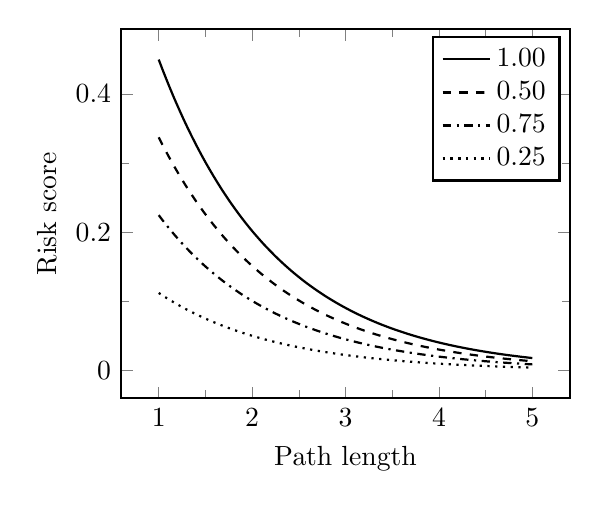
\begin{tikzpicture}
\begin{axis}[
  xlabel={Path length},
  ylabel={Risk score},
  minor tick num=1,
  width=0.6\textwidth,
  smooth,
  domain=1:5,
  y domain=0.01:1,
  samples=100,
  black,
  thick
]
  \addplot[] {e^(-0.8 * x)};
  \addplot[dashed] {0.75 * e^(-0.8 * x)};
  \addplot[dashdotted] {0.5 * e^(-0.8 * x)};
  \addplot[dotted] {0.25 * e^(-0.8 * x)};
  \legend{$1.00$, $0.50$, $0.75$, $0.25$};
\end{axis}
\end{tikzpicture}
\caption[Exponential decay of risk scores]{Exponential decay of risk scores.}
\label{fig:decay}
\end{figure}

%\section{System Model}\label{sec:system-model}

% TODO - security, privacy, mobile crowd-sensing
% TODO - PDAs vs local computation

%The system model is similar to that in previous work \citep{Ayday2020, Ayday2021}. \Cref{fig:actor-dataflow} illustrates the corresponding data flow\footnote{A \emph{data-flow diagram} consists of data processors (circles), directed data flow (arrows), data stores (parallel lines), and external entities (rectangles) \cite[pp. 437--438]{Fowler2004}\label{foot:dataflow}.}.
%
%\begin{itemize}
%    \item Each user owns a \emph{personal data store} (PDS), a form of cloud storage that empowers the user with ownership and access control over their data.
%    \item Symptom scores are computed in a user's PDS to support integrating multiple streams of personal data \citep{Ayday2020}. While local symptom-score computation \citep{Ayday2020, Ayday2021} is more privacy-preserving, it is assumed that the user's PDS is a trusted entity.
%    \item User device interactions serve as a proxy for proximal human interactions. This work does not assume a specific protocol, but does assume that the protocol can approximate the duration of contact with relative accuracy and that communication with the actors of those contacted users can be established in a privacy-preserving manner.
%    \item No geolocation data is collected \citep{Ayday2020}. As a decentralized, proximity-based solution, it is not necessary to collect user geolocation data. See \Cref{sec:location-based} for a discussion of a geolocation-based design that was considered.
%    \item Actor-based risk propagation is a distributed, online algorithm \cite[pp. 791--818]{Cormen2022}. Previous work \citep{Ayday2020, Ayday2021} (see also \Cref{sec:previous-designs}) formulates risk propagation as a centralized, offline algorithm that periodically aggregates all user data to estimate infection risk. To improve the privacy, scalability, and responsiveness of ShareTrace, this work designs risk propagation to avoid data aggregation and to estimate infection risk in near real-time.
%\end{itemize}
%
%\begin{figure}[htb]
%    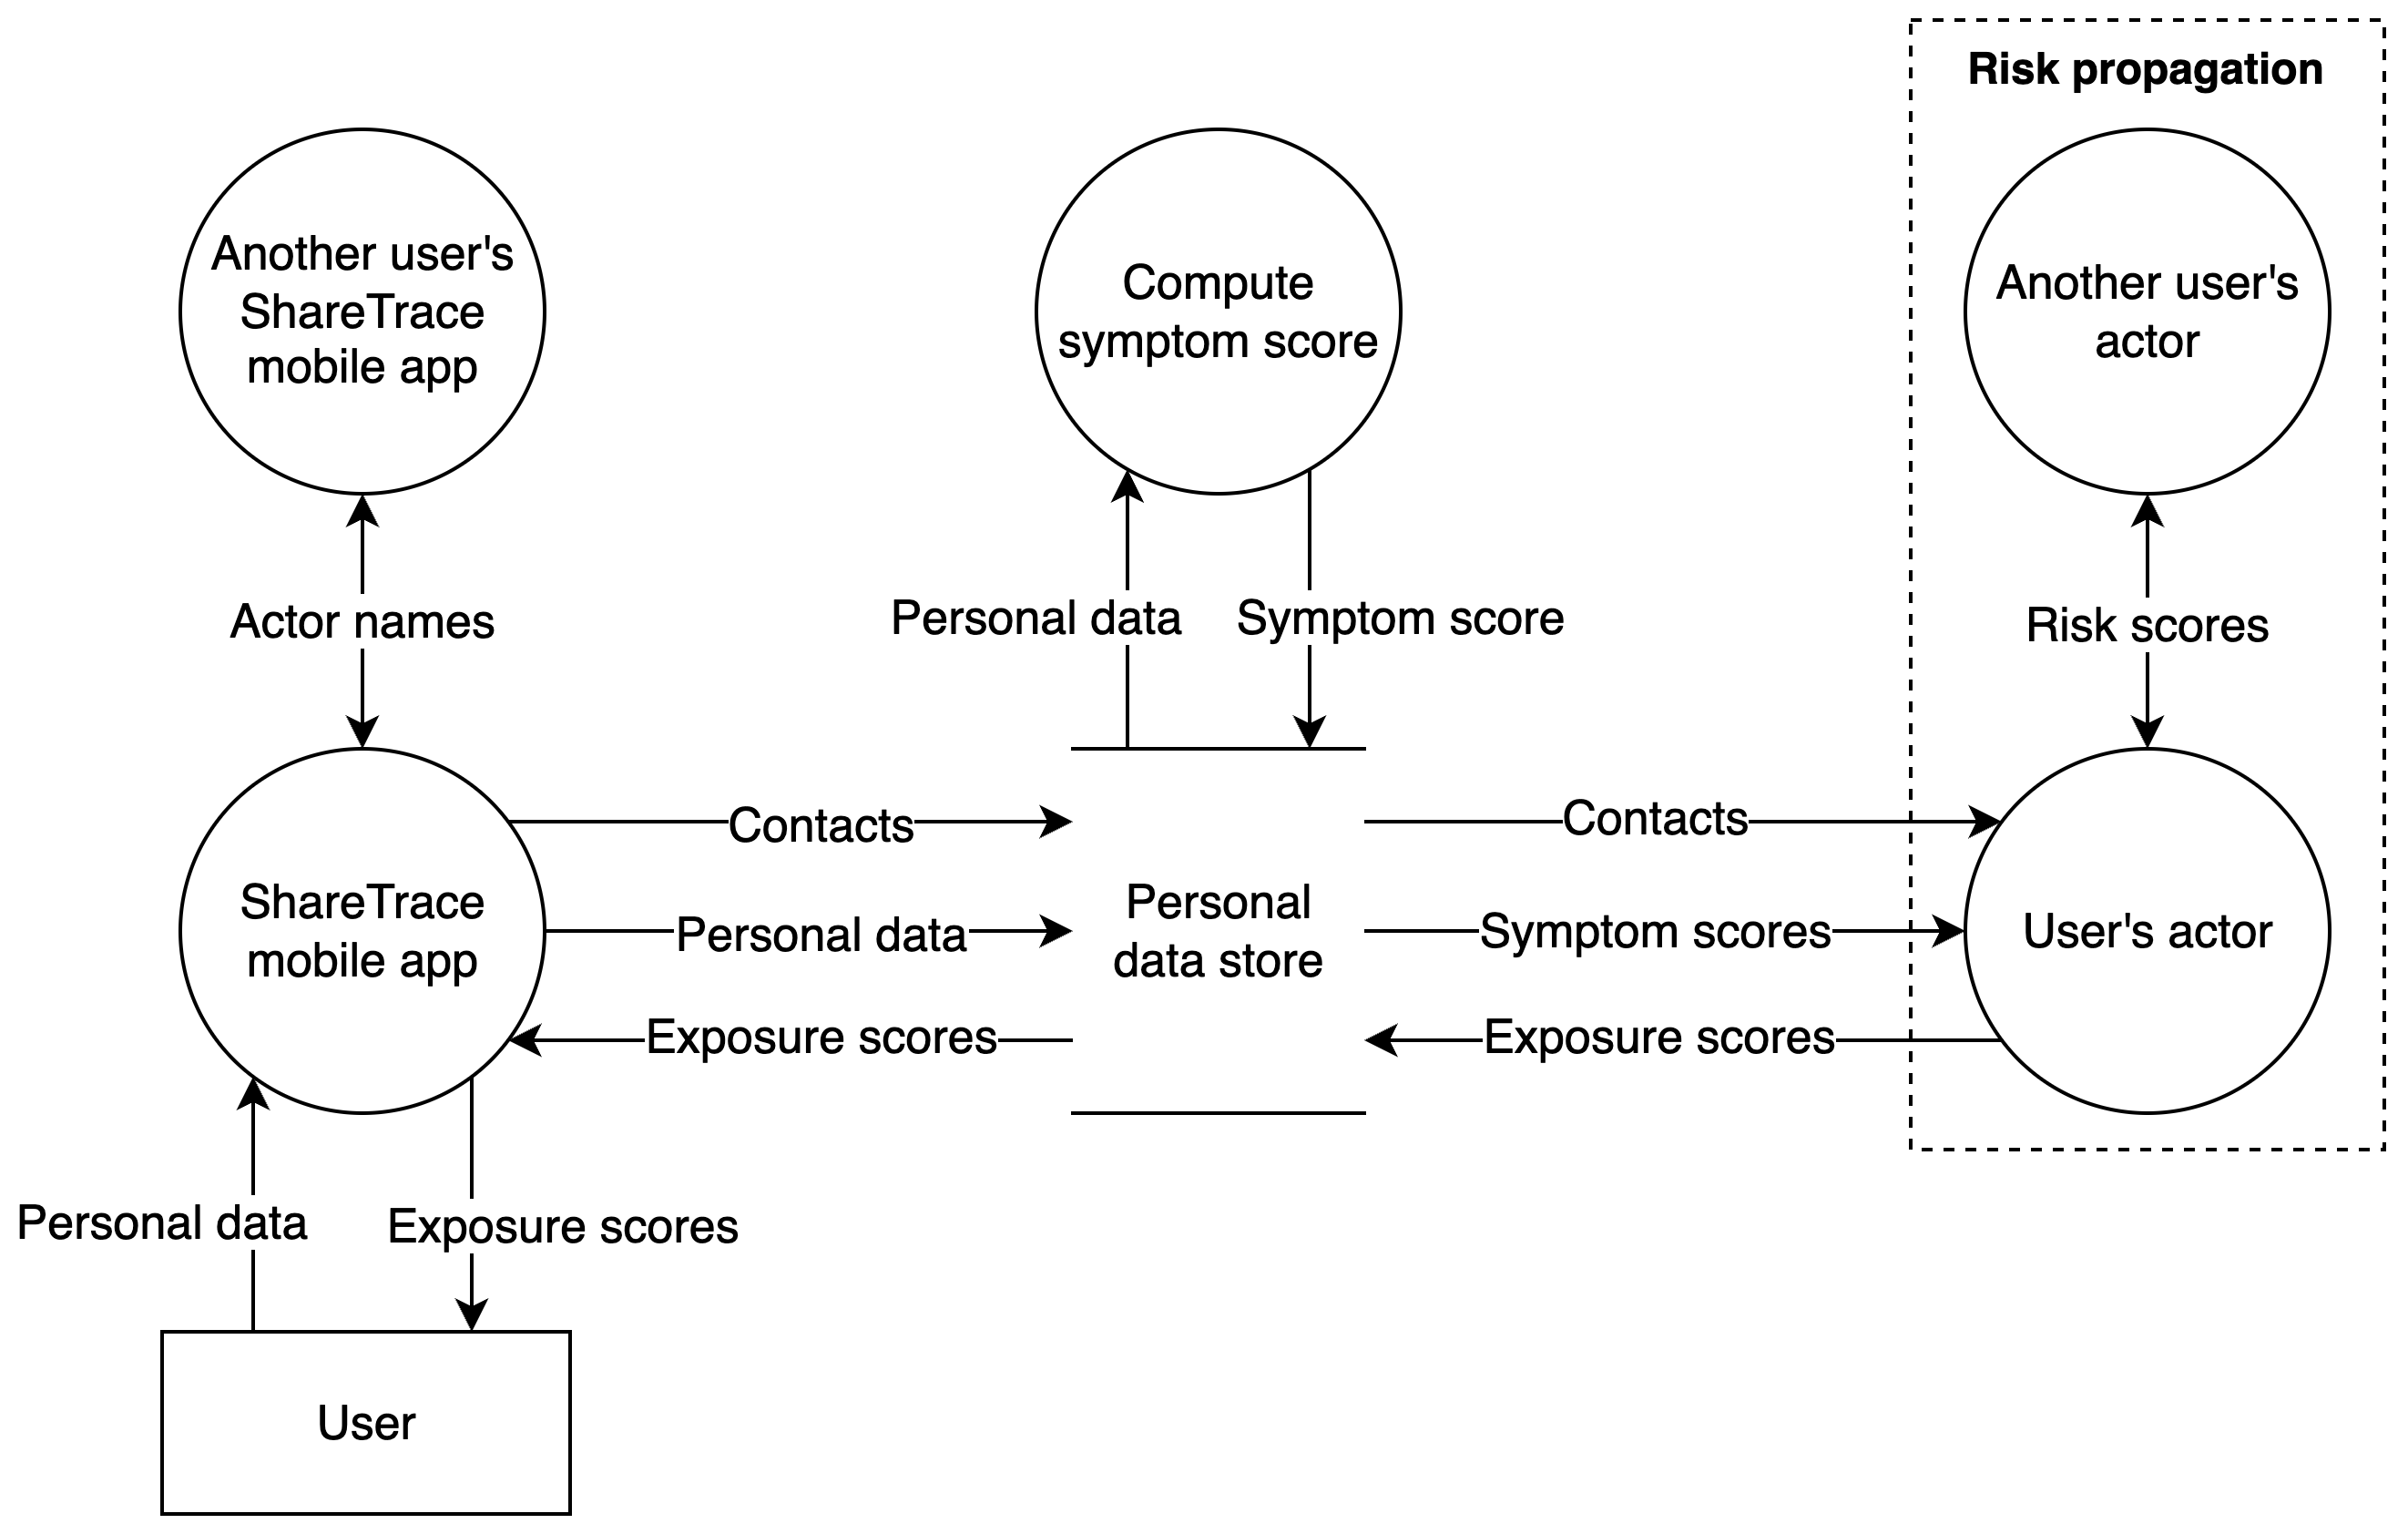
\includegraphics[width=\textwidth]{distributed-dataflow}
%    \caption[Distributed ShareTrace data flow]{Distributed ShareTrace data flow. \emph{Contacts} include the actor name and contact time of all users with which the user came into close proximity. \emph{Personal data} includes the user's demographics, reported symptoms, and diagnosis. It may also include machine-generated biomarkers and electronic health record data \citep{Ayday2020}.}
%    \label{fig:distributed-dataflow}
%\end{figure}
%
%\begin{figure}[htb]
%    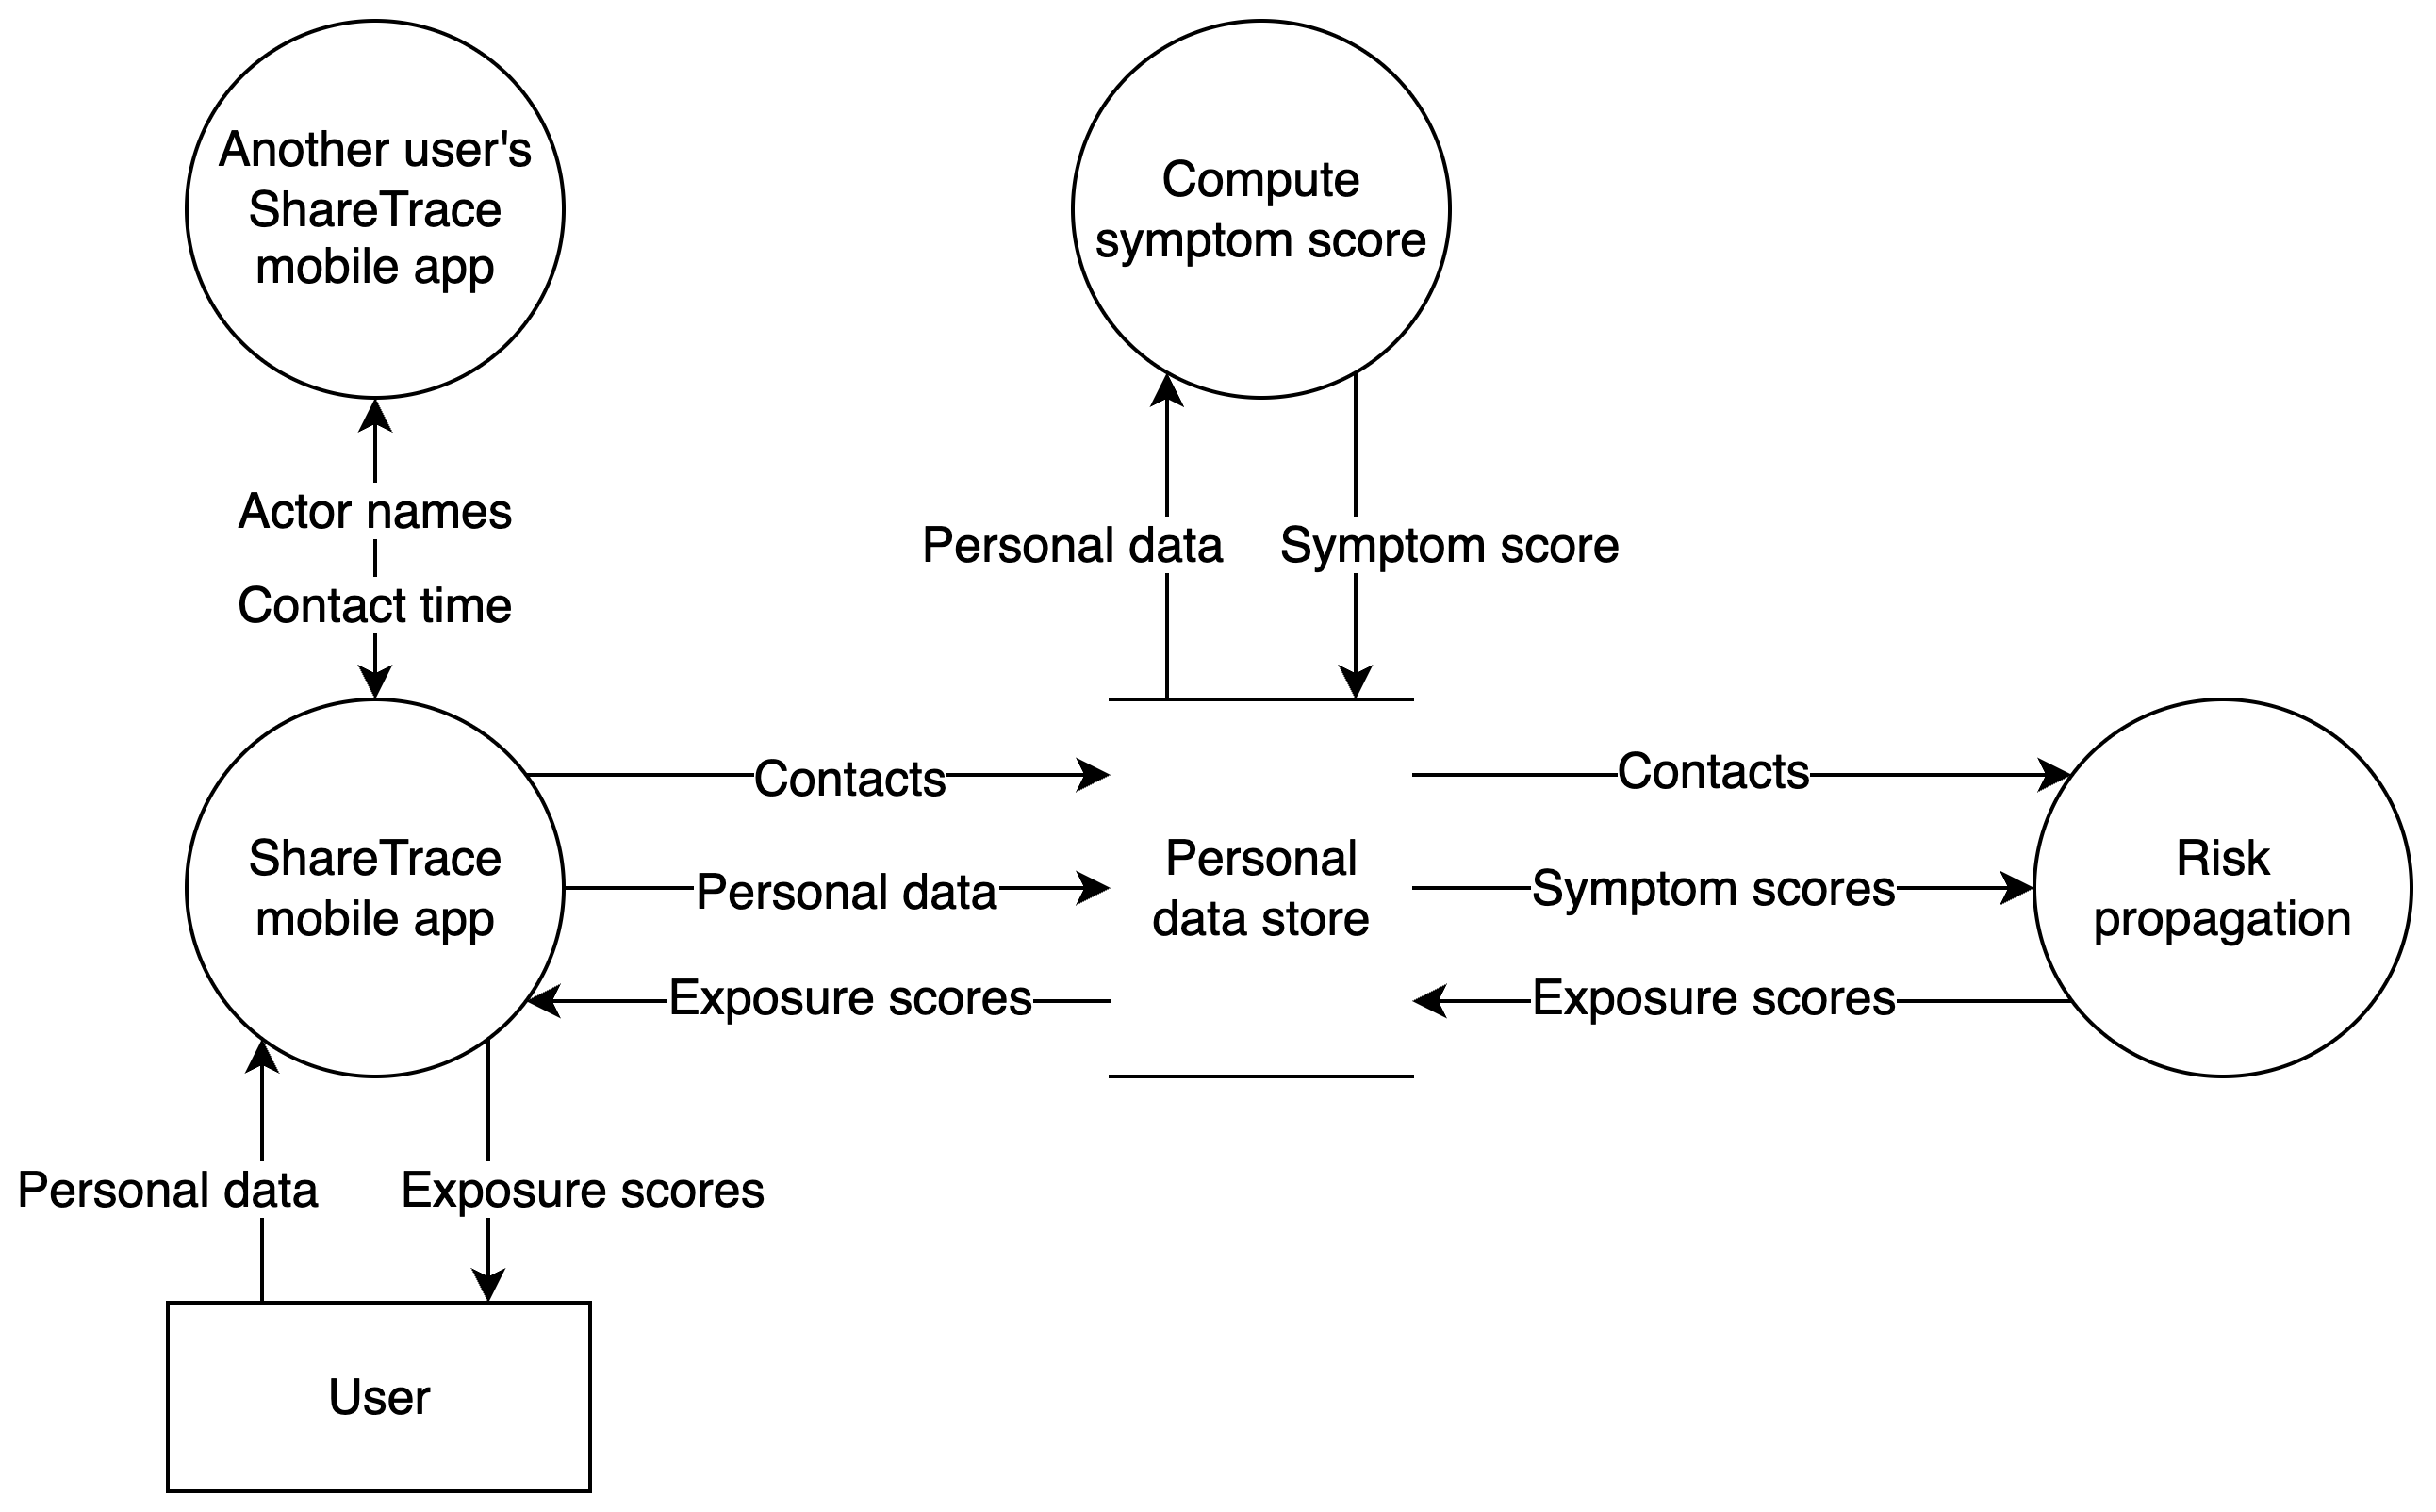
\includegraphics[width=\textwidth]{centralized-dataflow}
%    \caption[Centralized ShareTrace data flow]{Centralized ShareTrace data flow. \emph{Contacts} include the actor name and contact timestamp of all users with which the user came into close proximity. \emph{Personal data} includes the user's demographics, reported symptoms, and diagnosis. It may also include machine-generated biomarkers and electronic health record data \citep{Ayday2020}.}
%    \label{fig:centralized-dataflow}
%\end{figure}